This section describes the User interface of the CKB system, offering a glimpse into the various pages that constitute the website. The design mockups presented here prioritize the interaction dynamics rather than the final aesthetic design, recognizing that visual elements may get adjustments during the testing phase. Emphasizing the desktop browser version aligns with the system's primary purpose of facilitating code writing. However, it's important to note that equivalent pages will be tailored for the mobile version, ensuring a seamless user experience by appropriately rescaling and modifying the interface. As outlined in the RASD, the presented design mockups serve as a foundational representation, subject to refinement and optimization as the system evolves through testing and user feedback.

\section{Overview}

\begin{figure}[H]
    \begin{center}
        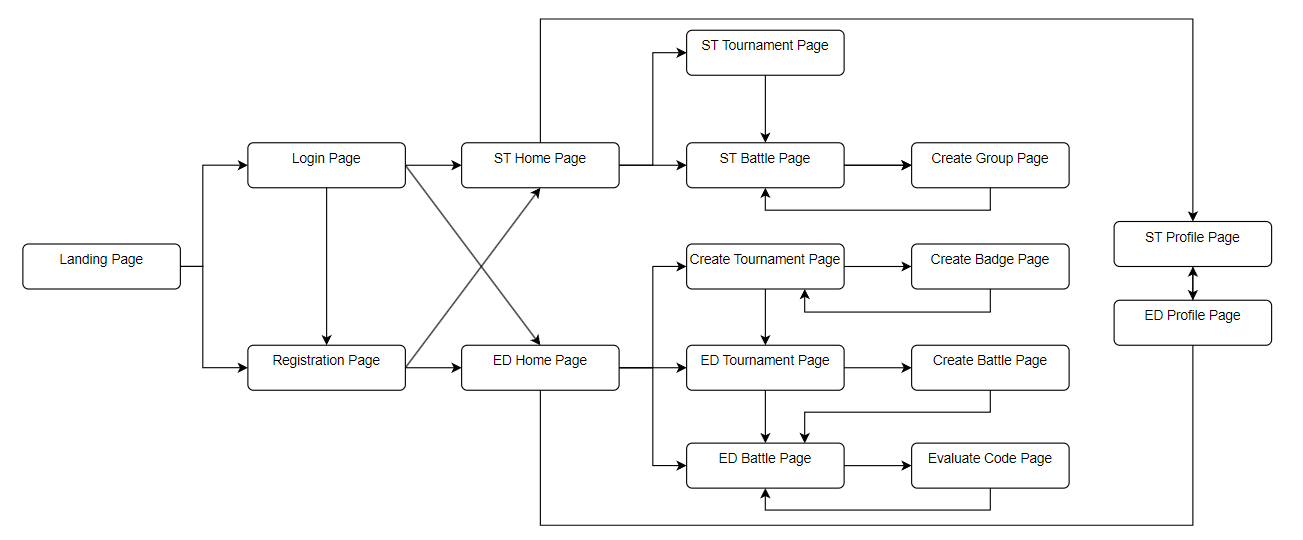
\includegraphics[width=1\linewidth]{Interfaces_UI/Overview_UID.png}
        \caption{User Interface Overview.}
        \label{fig:user_interface_overview}%
    \end{center}
\end{figure}

The provided image offers a comprehensive overview of the CKB system's pages, illustrating  their connections and pathways for user navigation. Each page is described in the sections below, except from the landing page that is implicit because it is a page where the User can only click on Login or Register. In order to better understand the entire image we didn’t connect the Tournament and Battle pages with the Profile pages. The schema above illustrates the correct workflow for a ST or an ED following all the passages from the login to every possible action.

\section{Header}

\begin{figure}[H]
    \begin{center}
        
\includegraphics[width=1\linewidth]{Interfaces_UI/Headline_UID.png}
        \caption{Header.}
        \label{fig:header}%
    \end{center}
\end{figure}

Across all pages in the CKB system, a uniform header ensures a consistent and user-friendly experience. Featuring the website name, User nickname, User icon for profile access, notification icon for updates, and a search bar for User and Tournament exploration, this cohesive design fosters familiarity and accessibility. The search bar is intentionally hidden on form pages to prevent potential interference with form responses. 

\newpage

\section{User Interfaces}
\newcounter{ui}
\setcounter{ui}{1}
\newcommand{\cui}{\theui\stepcounter{ui}}

\subsection*{UI\cui . Login and Registration Pages}

\begin{figure}[H]
    \begin{center}
        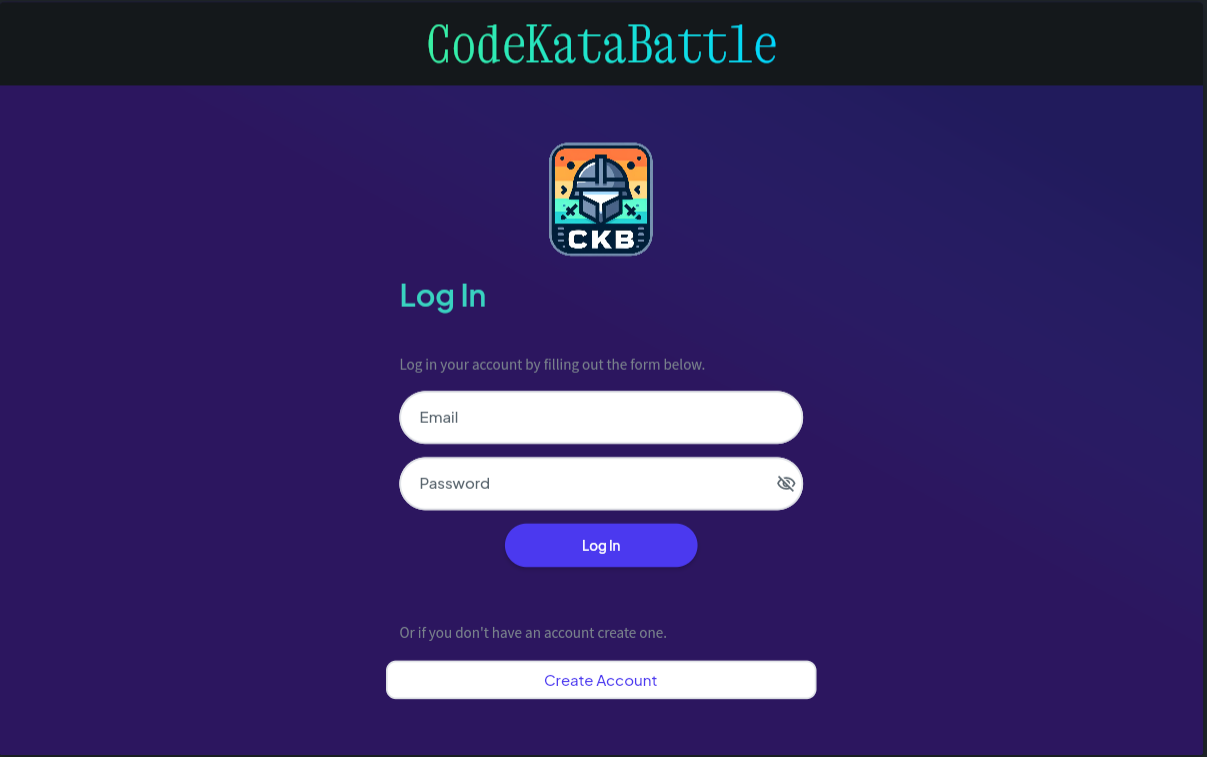
\includegraphics[width=0.7\linewidth]{Interfaces_UI/Login_UID.png}
        \caption{Login Page.}
        \label{fig:login_page}%
    \end{center}

    \begin{center}
        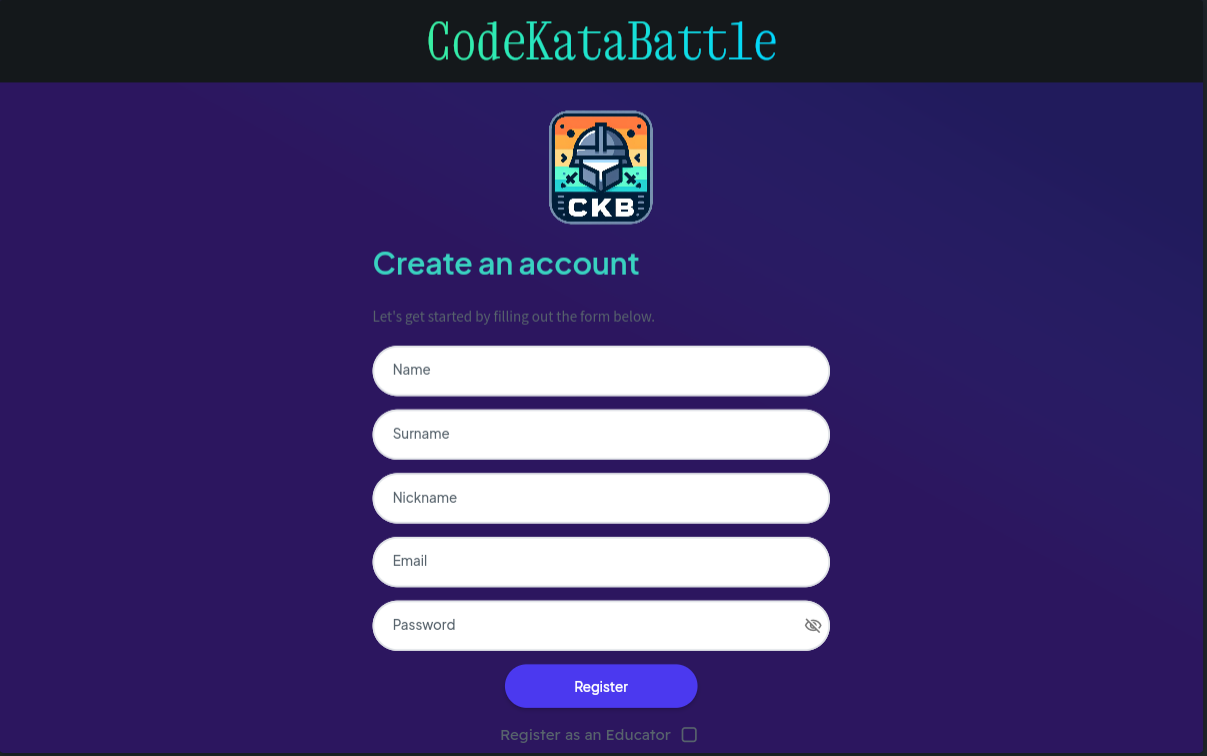
\includegraphics[width=0.7\linewidth]{Interfaces_UI/Registration_UID.png}
        \caption{Registration Page.}
        \label{fig:registration_page}%
    \end{center}
\end{figure}

The “Login” and the “Registration” pages are simple form pages where the Users insert their credentials that will be checked by the system before refreshing to the “ED Homepage” or “ST Homepage”. In the registration page the ED have to check the “Register as an Educator” box to inform CKB that they need ED’s permission to create and manage Tournaments and Battles. 

\subsection*{UI\cui . ED Homepage}

\begin{figure}[H]
    \begin{center}
        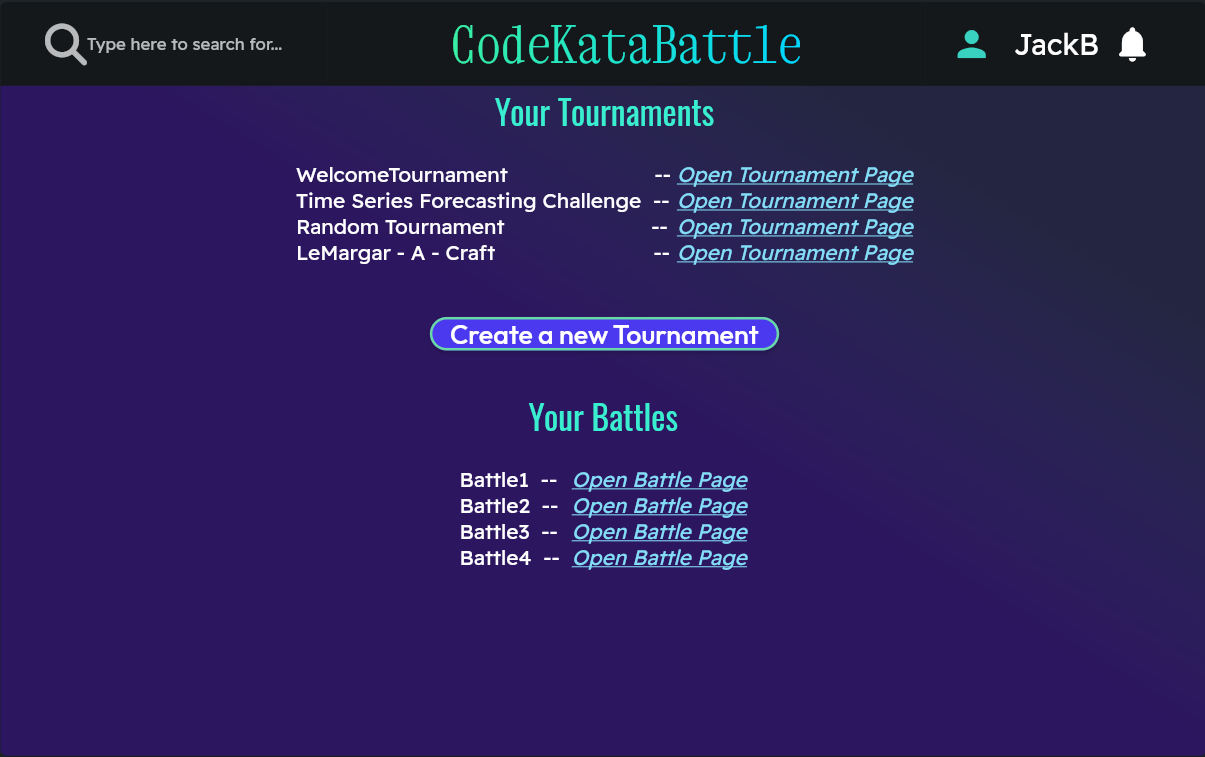
\includegraphics[width=0.7\linewidth]{Interfaces_UI/ED_Home_UID.png}
        \caption{ED Homepage.}
        \label{fig:ed_homepage}%
    \end{center}
\end{figure}

From the “Login” and “Registration” pages the ED will be redirected to the “ED Homepage”. From here the ED can visualize his own Tournaments and Battles previously created and create new Tournaments to let the STs participate in new challenges.

\subsection*{UI\cui . Create Tournament Page}

\begin{figure}[H]
    \begin{center}
        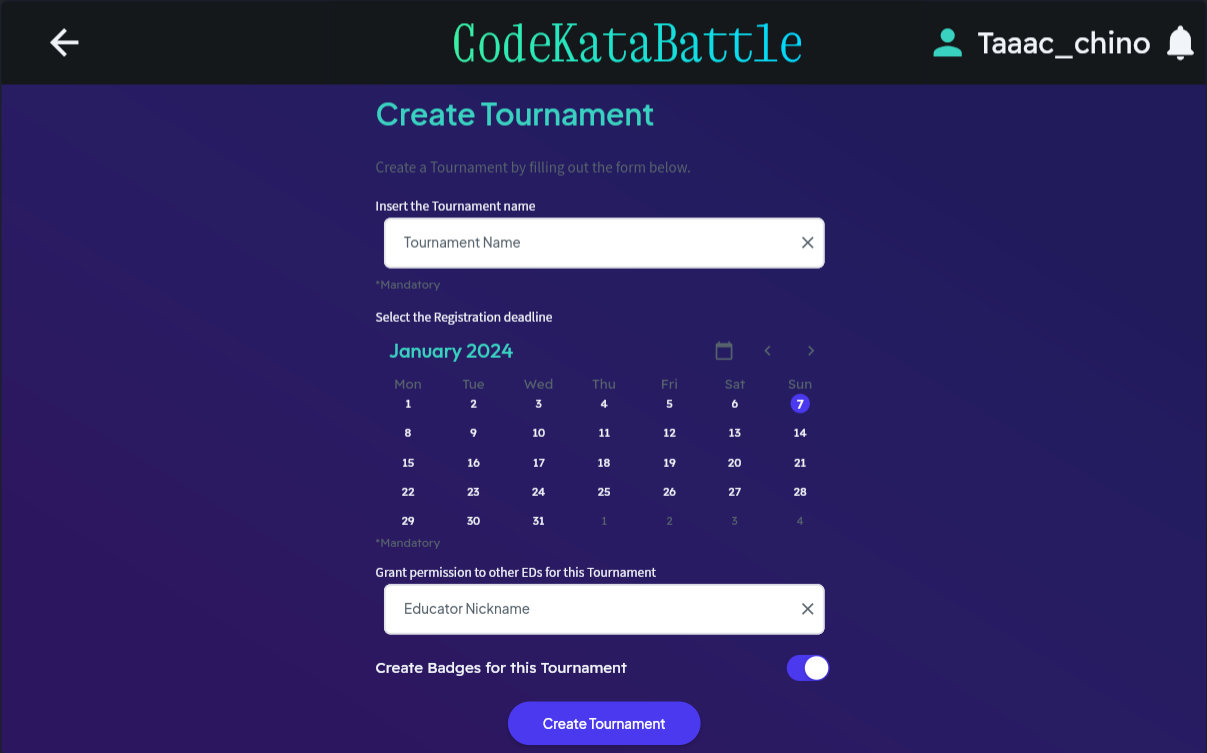
\includegraphics[width=0.7\linewidth]{Interfaces_UI/CreateTournament_UID.png}
        \caption{Create Tournament Page.}
        \label{fig:create_tournament_page}%
    \end{center}
\end{figure}

The “Create Tournament” form page is where the ED  input mandatory parameters and have the option to grant to other EDs permissions to create Battles within the Tournament. An additional checkbox allows EDs to indicate whether they want to create or modify Badges associated with the Tournament. CKB checks the input parameters before refreshing to the “ED Tournament” page or to the “Create Badge” page.

\subsection*{UI\cui . Create Badge Page}

\begin{figure}[H]
    \begin{center}
        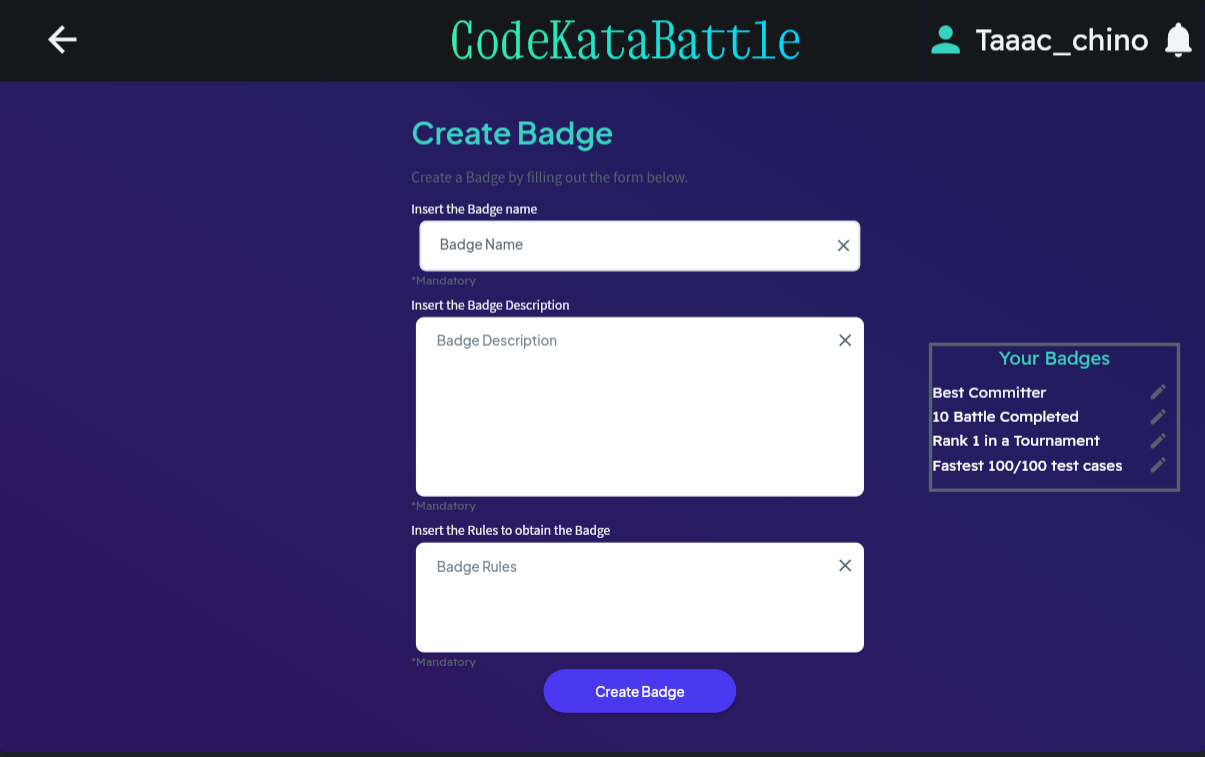
\includegraphics[width=0.7\linewidth]{Interfaces_UI/CreateBadge_UID.png}
        \caption{Create Badge Page.}
        \label{fig:create_badge_page}%
    \end{center}
\end{figure}

If the ED has checked the Badge creation box the “Create Badge” form page will be shown to him to let the ED create new Badges with their description and the rules to obtain them. In this page the ED can also check the previously created Badge for his other Tournaments and modify them if wanted.

\subsection*{UI\cui . ED Tournament Page}

\begin{figure}[H]
    \begin{center}
        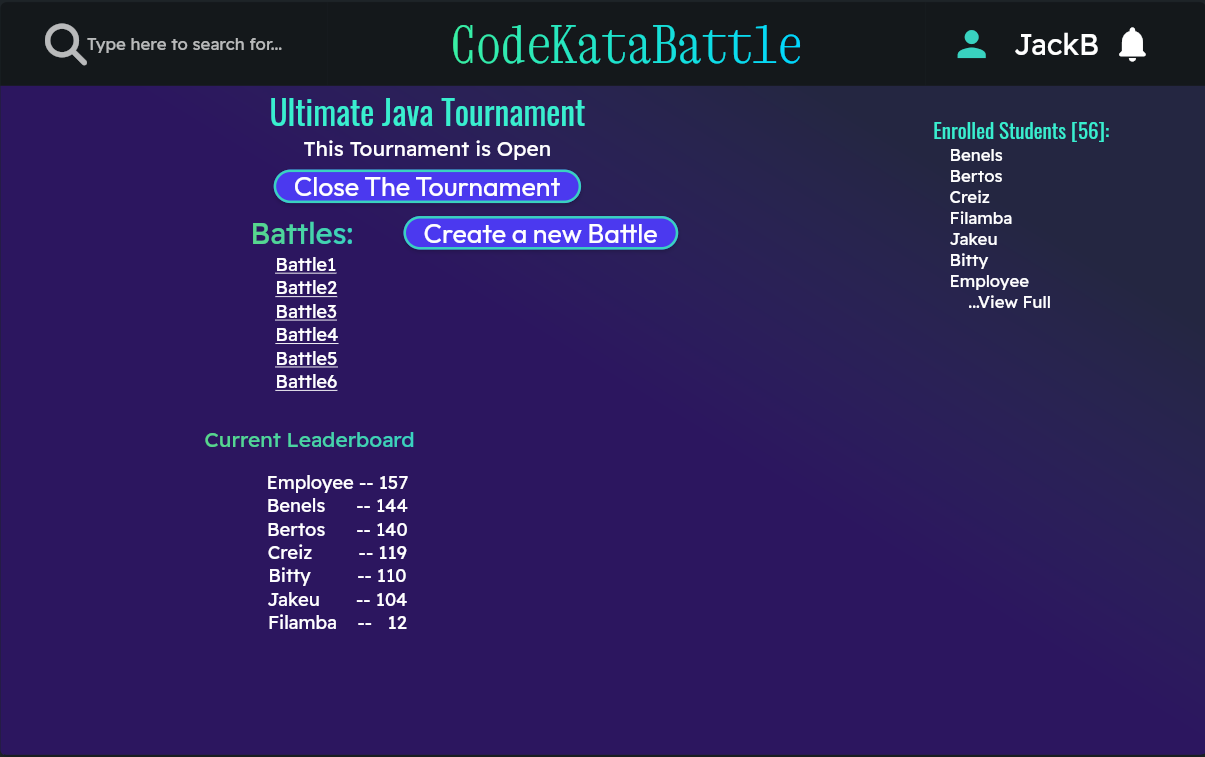
\includegraphics[width=0.7\linewidth]{Interfaces_UI/ED_Tour_UID.png}
        \caption{ED Tournament Page.}
        \label{fig:ed_tournament_page}%
    \end{center}   
\end{figure}

In the “ED Tournament” page the ED can check the Tournament that it has created where it is shown the Leaderboard with each ST that has subscribed to the Tournament and from this page it can create new Battles by clicking the “Create Battle” button.

\subsection*{UI\cui . Create Battle Page}

\begin{figure}[H]
    \begin{center}
        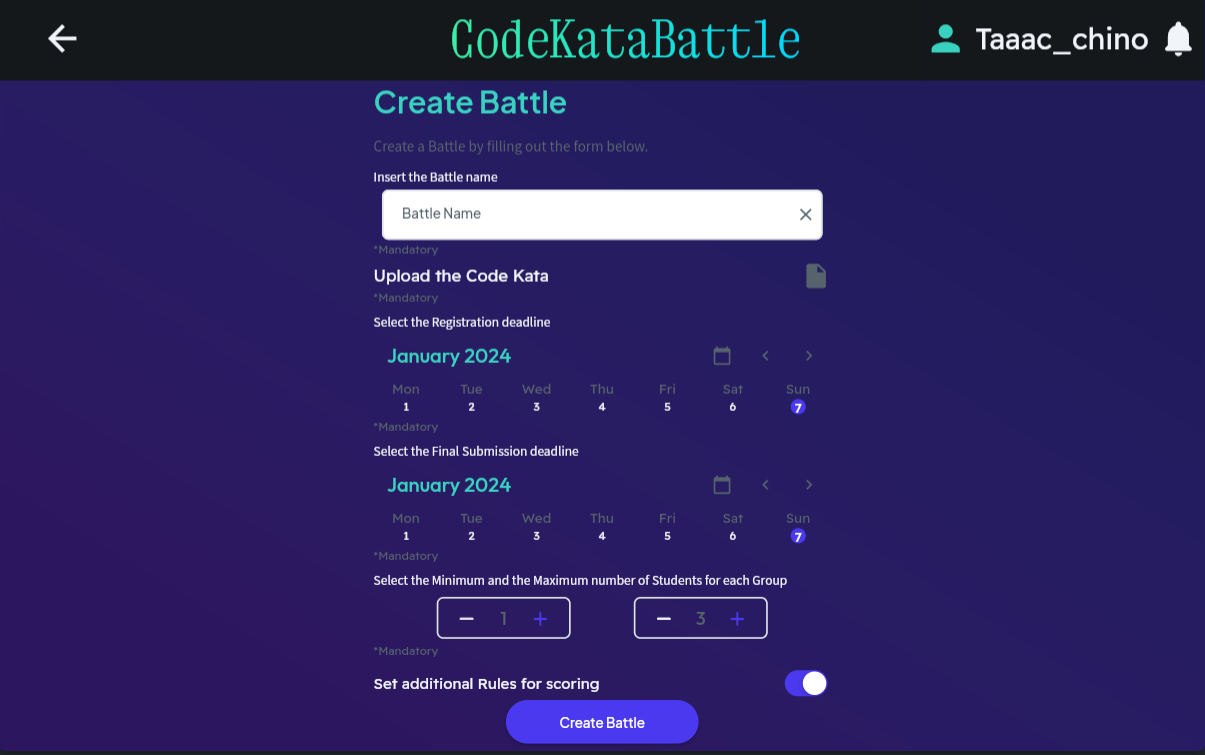
\includegraphics[width=0.7\linewidth]{Interfaces_UI/CreateBattle_UID.png}
        \caption{Create Battle Page.}
        \label{fig:create_battle_page}%
    \end{center}
\end{figure}

The “Create Battle” page is the form where the ED inserts the parameters to create a new Battle -the mandatory ones need to be inputted to create the Battle- and when the “Create Battle” button is clicked by the ED a notification is sent to all the ST subscribed to the Tournament.

\subsection*{UI\cui . ED Battle Page}

\begin{figure}[H]
    \begin{center}
        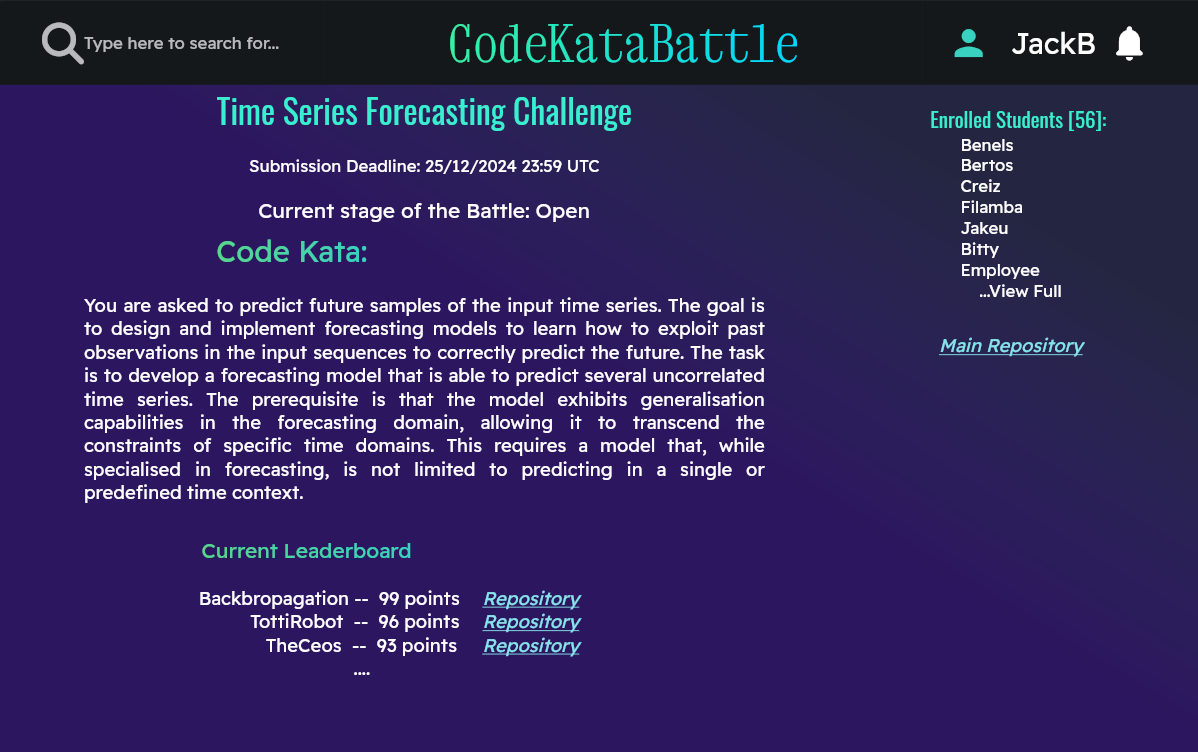
\includegraphics[width=0.7\linewidth]{Interfaces_UI/ED_Battle_Leaderboard_UID.png}
        \caption{ED Battle Page.}
        \label{fig:ed_battle_page}%
    \end{center}
\end{figure}

The “ED Battle” page shows the most concerning data about the Battle, such as the submission deadline and the code kata. In this page, also the current leaderboard of the Battle is shown and the ED can view a full list of the STs enrolled in the Battle. The ED might click on the proper link to get redirected to a certain STG’s repository. In the same section, when the Battle stage is set to the ‘Consolidation Stage’, the ED can also manually evaluate the STGs’ works.

\subsection*{UI\cui . Evaluate Code Page}

\begin{figure}[H]
    \begin{center}
        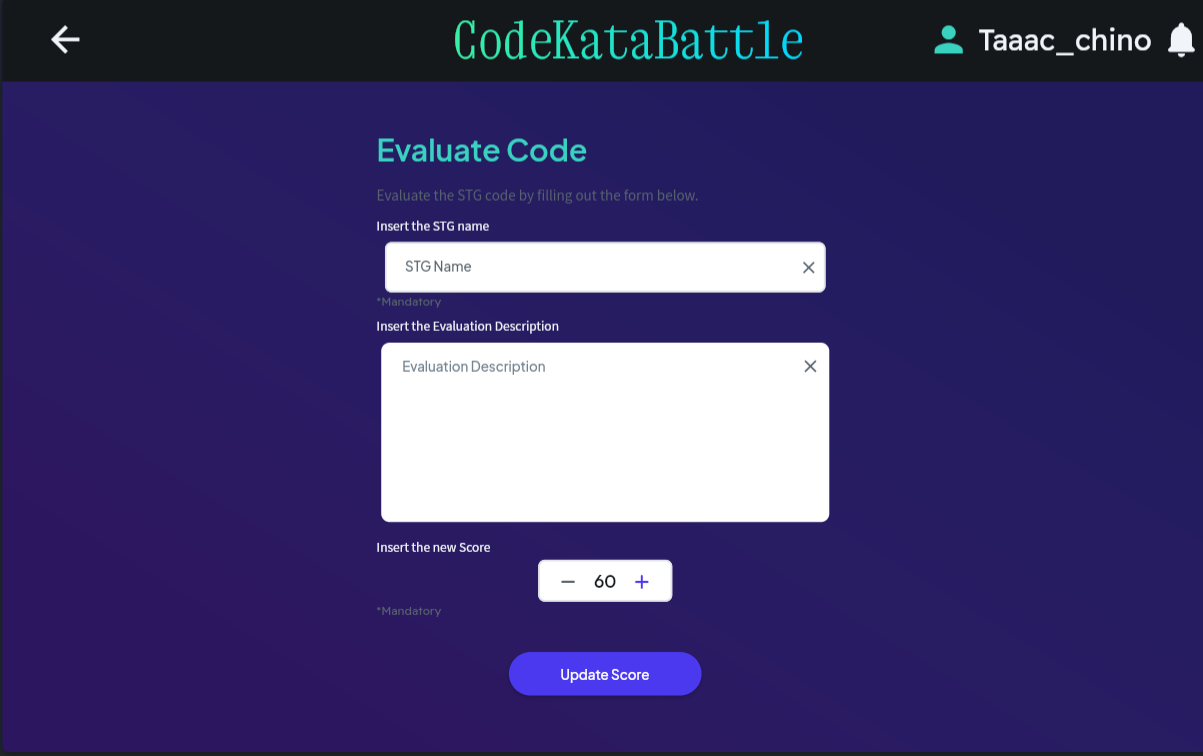
\includegraphics[width=0.7\linewidth]{Interfaces_UI/EvaluateCode_UID.png}
        \caption{Evaluate Code Page.}
        \label{fig:evaluate_code_page}%
    \end{center}   
\end{figure}

The “Evaluate Code” page is used when the ED wants to manually evaluate the STGs’ code during the ‘Consolidation Stage’ of a Battle. The ED is able to manually update the score and write some comments about the code for a certain STG. 

\subsection*{UI\cui . ST Homepage}

\begin{figure}[H]
    \begin{center}
        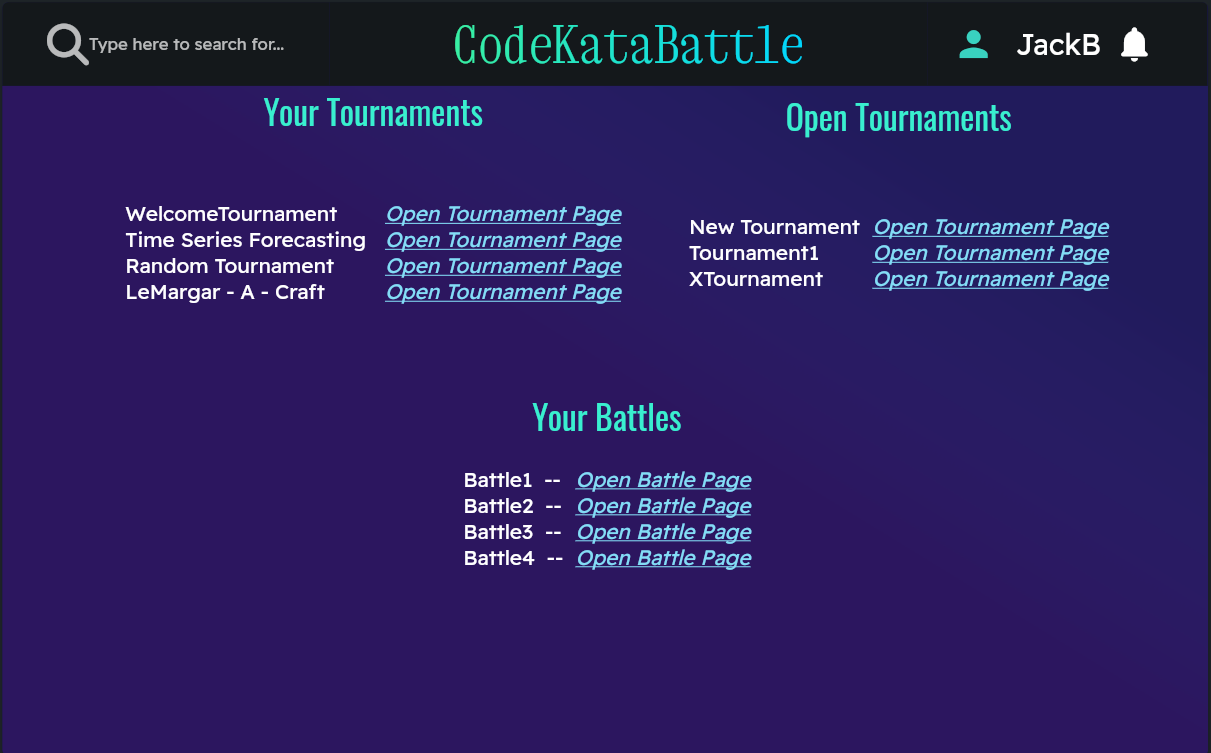
\includegraphics[width=0.7\linewidth]{Interfaces_UI/ST_home_UID.png}
        \caption{ST Homepage.}
        \label{fig:st_homepage}%
    \end{center}
\end{figure}

The “ST Homepage” is the main page where the ST can visualize his ongoing Tournaments with the respective Battles, but also checks any other Tournament that have been created on CKB. 

\subsection*{UI\cui . ST Tournament Page}

\begin{figure}[H]
    \begin{center}
        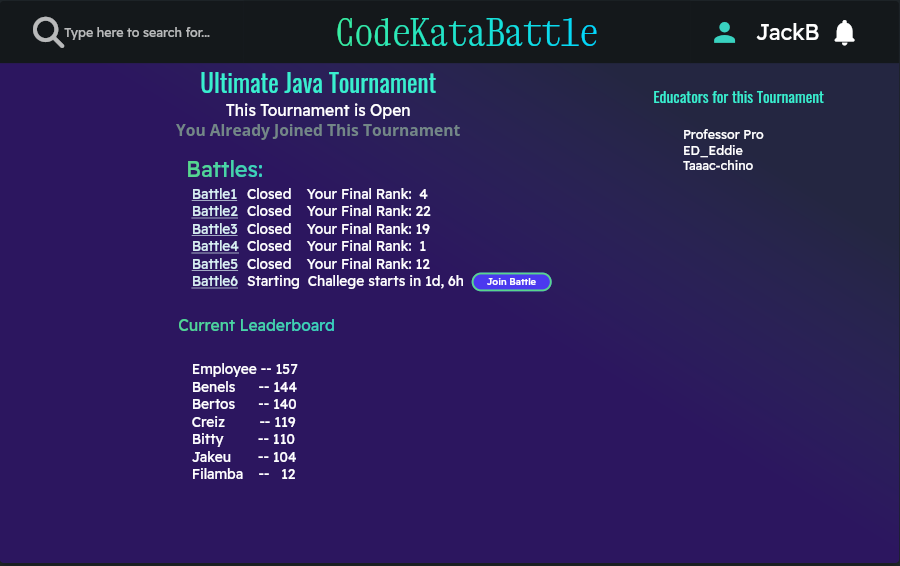
\includegraphics[width=0.7\linewidth]{Interfaces_UI/ST_Tour_v2.png}
        \caption{ST Tournament Page.}
        \label{fig:st_tournament_page}%
    \end{center}
\end{figure}

In the "ST Tournament” page the ST can check all the information about this ongoing Tournament, such as the Battles, the EDs and the leaderboard, and join new Battles when they are created.

\subsection*{UI\cui . Create Group Page}

\begin{figure}[H]
    \begin{center}
        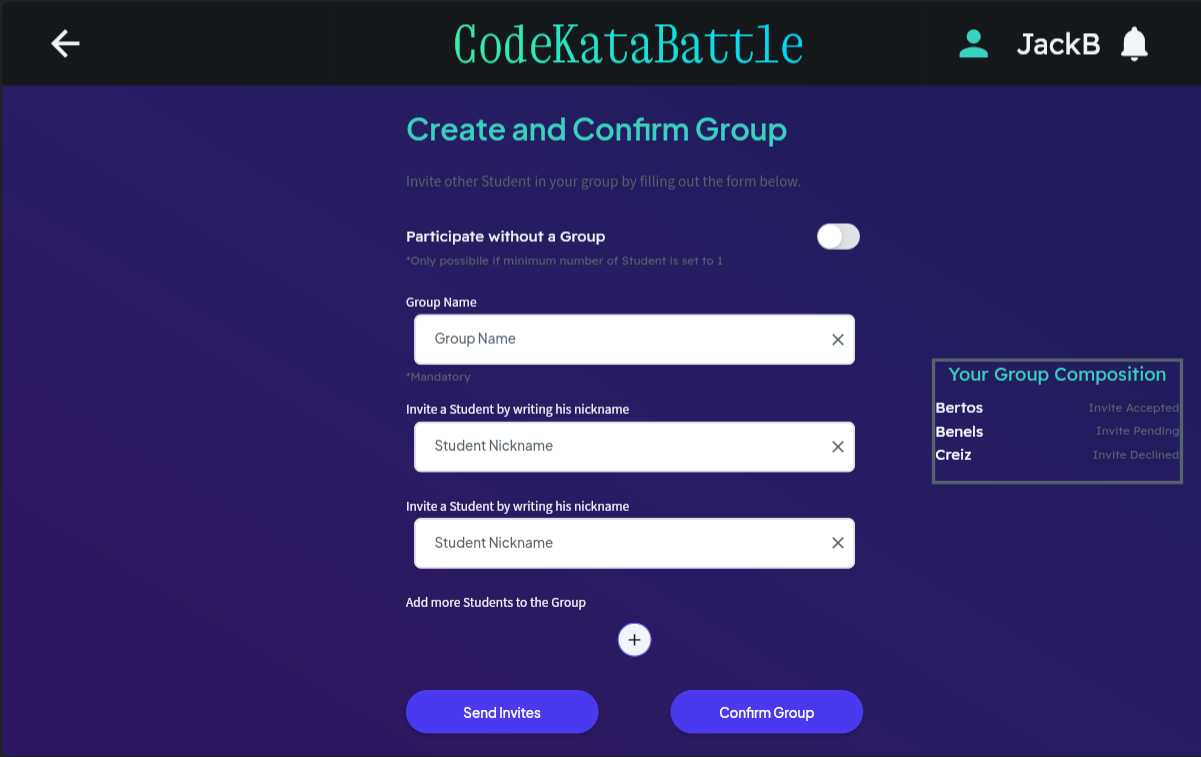
\includegraphics[width=0.7\linewidth]{Interfaces_UI/CreateGroup_UID.png}
        \caption{Create Group Page.}
        \label{fig:create_group_page}%
    \end{center}
\end{figure}

The “Create Group” page is used by the ST to create and confirm a STG within a Battle. After inserting the name of the STG, the ST can invite other mutuals to join his group by writing their nickname in the proper box and then clicking on the “Send Invites” button. Once the STs accepted the invites and the STG is full, the ST that acts as the creator of the Group can click on the “Confirm Group” button in order to successfully end the STG creation process. 

\subsection*{UI\cui . ST Battle Page}  

\begin{figure}[H]
    \begin{center}
        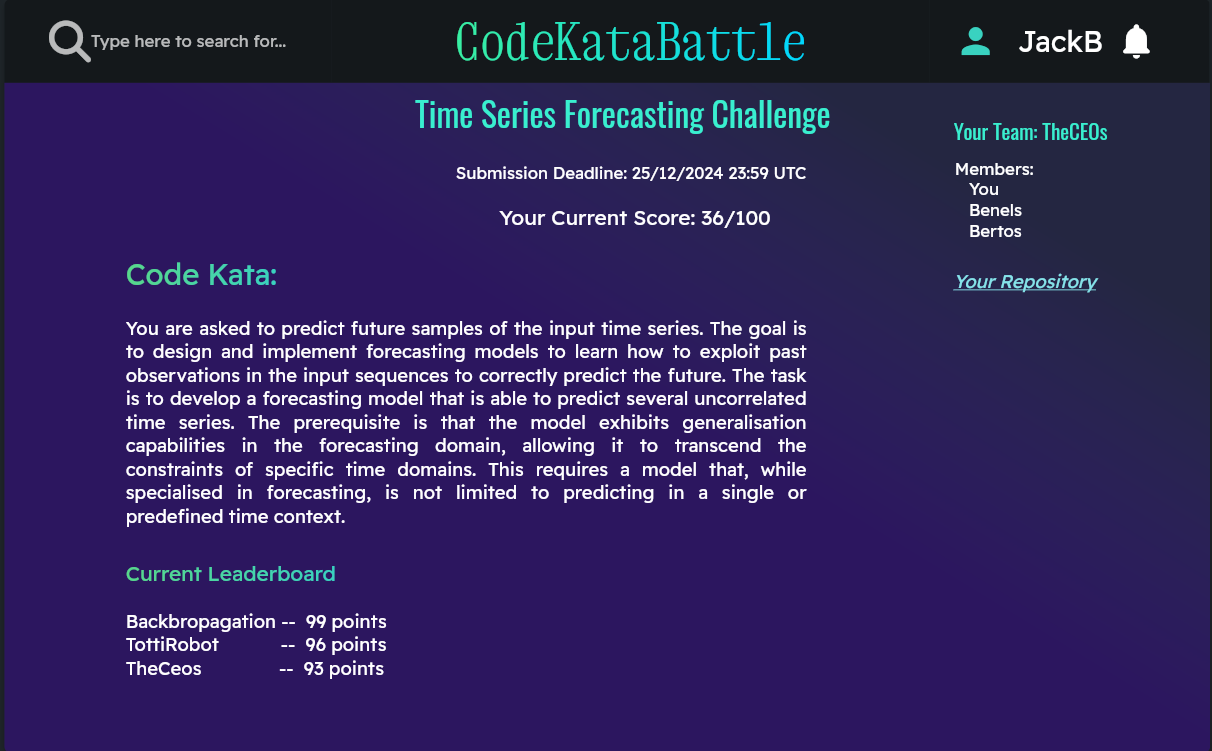
\includegraphics[width=0.7\linewidth]{Interfaces_UI/ST_Battle_UID.png}
        \caption{ST Battle Page.}
        \label{fig:st_battle_page}%
    \end{center}
\end{figure}

This is the "ST Battle" page. Here CKB will show the name of the Battle, the submission deadline and the code kata. The page will also show the current leaderboard and the group of the ST, alongside with the link to the STG’s repository.

\subsection*{UI\cui . ED and ST Pofile Pages}

\begin{figure}[H]
    \begin{center}
        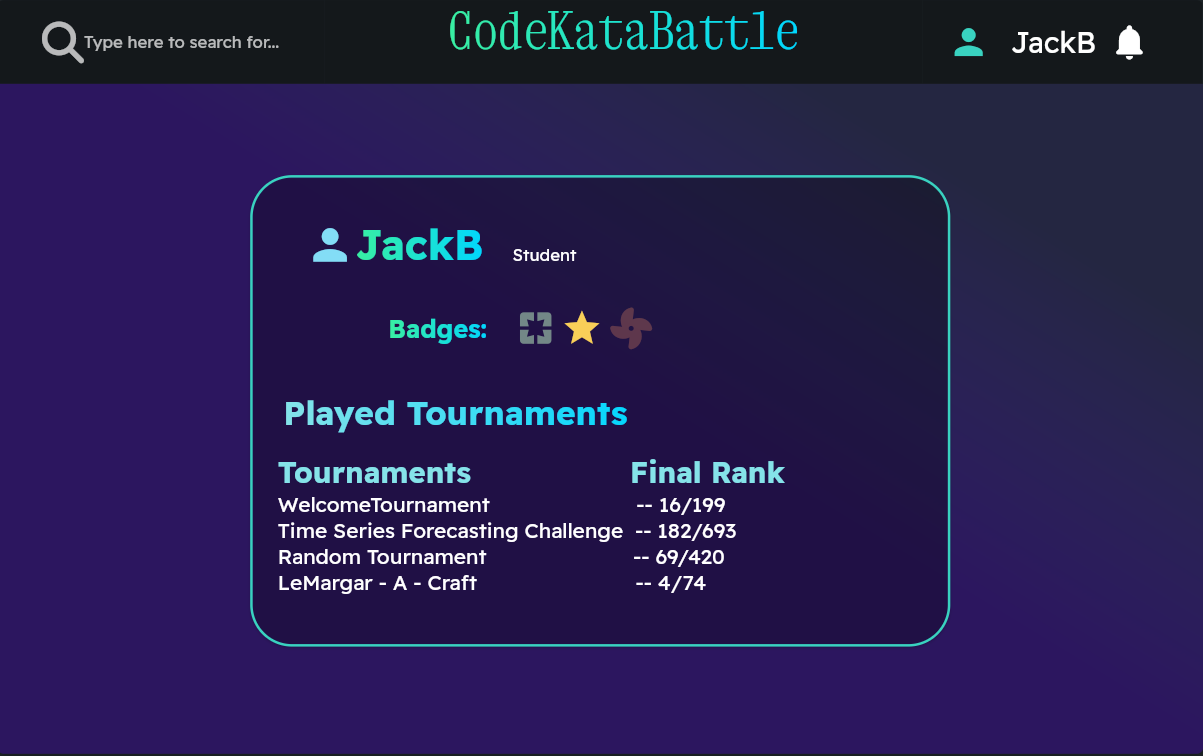
\includegraphics[width=0.7\linewidth]{Interfaces_UI/ST_profile_UID.png}
        \caption{ST Profile Page.}
        \label{fig:st_profile_page}%
    \end{center}

    \begin{center}
        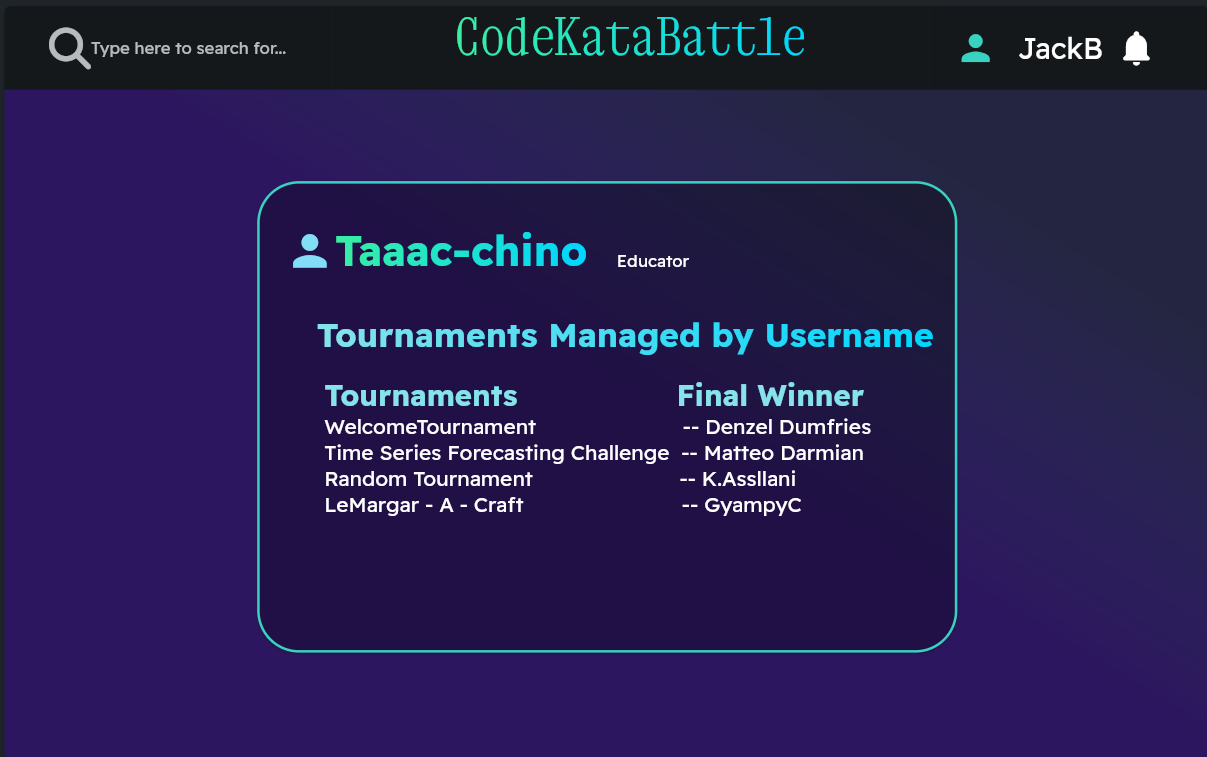
\includegraphics[width=0.7\linewidth]{Interfaces_UI/ED_profile_UID.png}
        \caption{ED Profile Page.}
        \label{fig:ed_profile_page}%
    \end{center}
\end{figure}

The Profile Pages show the details of a User, whether he is a ST or an ED. In both of the profiles, the page will show the Nickname, the profile picture and the role, with this being ‘Student’ or ‘Educator’. In the first case the page will show all the badges awarded to the ST alongside the Tournaments that he played and the respective final results. In the second case, the page will only show in addition the last Tournaments managed by this ED.



